\documentclass[conference]{IEEEtran}
\usepackage{cite}
\usepackage[pdftex]{graphicx}
\usepackage{fancybox}
\usepackage{tikz}
\usepackage{tikz-qtree}
\usetikzlibrary{shadows,trees}
\usepackage[ruled,vlined]{algorithm2e}
\usepackage[cmex10]{amsmath}
\usepackage{array}
\usepackage{mdwmath}
\usepackage{mdwtab}
\usepackage{eqparbox}
\usepackage[tight,footnotesize]{subfigure}
\usepackage[caption=false,font=footnotesize]{subfig}
\usepackage{fixltx2e}
\usepackage{stfloats}
%\usepackage{hyperref}

% stfloats.sty was written by Sigitas Tolusis. This package gives LaTeX2e
% the ability to do double column floats at the bottom of the page as well
% as the top. (e.g., "\begin{figure*}[!b]" is not normally possible in
% LaTeX2e). It also provides a command:
%\fnbelowfloat
% to enable the placement of footnotes below bottom floats (the standard
% LaTeX2e kernel puts them above bottom floats). This is an invasive package
% which rewrites many portions of the LaTeX2e float routines. It may not work
% with other packages that modify the LaTeX2e float routines. The latest
% version and documentation can be obtained at:
% http://www.ctan.org/tex-archive/macros/latex/contrib/sttools/
% Documentation is contained in the stfloats.sty comments as well as in the
% presfull.pdf file. Do not use the stfloats baselinefloat ability as IEEE
% does not allow \baselineskip to stretch. Authors submitting work to the
% IEEE should note that IEEE rarely uses double column equations and
% that authors should try to avoid such use. Do not be tempted to use the
% cuted.sty or midfloat.sty packages (also by Sigitas Tolusis) as IEEE does
% not format its papers in such ways.
\hyphenation{op-tical net-works semi-conduc-tor}

\begin{document}
%
% paper title
% can use linebreaks \\ within to get better formatting as desired
\title{Search for MUMs in enhanced suffix tree traversal with SIMD instructions.}


% author names and affiliations
% use a multiple column layout for up to three different
% affiliations
\author{\IEEEauthorblockN{Julio C\'esar Garc\'ia Vizca\'ino}
\IEEEauthorblockA{Computer Architecture \& Operating Systems Department\\
Universitat Aut\`onoma de Barcelona\\
Bellaterra (Barcelona), Spain\\
Email: jcgarcia@caos.uab.cat}}
%\and
%\IEEEauthorblockN{}
%\IEEEauthorblockA{Twentieth Century Fox\\
%Springfield, USA\\
%Email: homer@thesimpsons.com}
%\and
%\IEEEauthorblockN{James Kirk\\ and Montgomery Scott}
%\IEEEauthorblockA{Starfleet Academy\\
%San Francisco, California 96678-2391\\
%Telephone: (800) 555--1212\\
%Fax: (888) 555--1212}}

% conference papers do not typically use \thanks and this command
% is locked out in conference mode. If really needed, such as for
% the acknowledgment of grants, issue a \IEEEoverridecommandlockouts
% after \documentclass

% for over three affiliations, or if they all won't fit within the width
% of the page, use this alternative format:
% 
%\author{\IEEEauthorblockN{Michael Shell\IEEEauthorrefmark{1},
%Homer Simpson\IEEEauthorrefmark{2},
%James Kirk\IEEEauthorrefmark{3}, 
%Montgomery Scott\IEEEauthorrefmark{3} and
%Eldon Tyrell\IEEEauthorrefmark{4}}
%\IEEEauthorblockA{\IEEEauthorrefmark{1}School of Electrical and Computer Engineering\\
%Georgia Institute of Technology,
%Atlanta, Georgia 30332--0250\\ Email: see http://www.michaelshell.org/contact.html}
%\IEEEauthorblockA{\IEEEauthorrefmark{2}Twentieth Century Fox, Springfield, USA\\
%Email: homer@thesimpsons.com}
%\IEEEauthorblockA{\IEEEauthorrefmark{3}Starfleet Academy, San Francisco, California 96678-2391\\
%Telephone: (800) 555--1212, Fax: (888) 555--1212}
%\IEEEauthorblockA{\IEEEauthorrefmark{4}Tyrell Inc., 123 Replicant Street, Los Angeles, California 90210--4321}}

%\IEEEspecialpapernotice{(Invited Paper)}

\maketitle

\begin{abstract}
 A suffix tree is a data structure very known to solve many classic string matching problems. One problem that can be solved with a suffix tree is the MUM-problem which is found in the MUMmer application. However, the search for MUMs presents challenges due to irregular and unpredictable data accesses in the suffix tree traversal. This paper enhances the traversal of a suffix tree by using contiguous nodes of suffix tree in depth levels and finding the correct child with a SIMD instruction. This little tweak allows having a reduction of search for MUMs time about 18\%. Moreover an evaluation of search for MUMs in multicore architectures is reviewed and compared with this enhanced traversal which has a better speedup.
\end{abstract}
\IEEEpeerreviewmaketitle

\section{Introduction}
Firstly, we define the MUM-problem. Assume we are given an alphabet $\Sigma^*$, two sequences R, Q $\in \Sigma^*$, and a number L $>$ 0. The maximal unique matches problem (MUM-problem) is to find all sequences u $\in \Sigma^*$ with: $|u|\geq L$, u occurs exactly once in R and once in Q, and for any character a $\in \Sigma^*$ neither ua nor au occurs both in R and Q.

Let's assume the Reference sequence $R[0,\ldots, n-1]$ of size $|R|=n$ over an alphabet $\Sigma={ \$, A, C, G, T}$ which has a sentinel character $R[n-1] = \$$ that occurs nowhere else in the Reference genome and is lexicographically less than all the characters that occur in the alphabet. The suffixes of the Reference genome are zero indexed by their position in the original Reference by a full-text index data structure like a suffix tree. 

\newtheorem{mydef}{Definition}
\begin{mydef}
A suffix tree, $ST$, for an n-character string $R$ is a rooted directed tree with exactly $n$ leaves numbered 0 to n. Each internal node, other than the root, has at least two children and each edge is labeled with a nonempty substring of $R$. No two edges out of a node can have edge-labels beginning with the same character. For any leaf $i$, the concatenation of the edge-labels on the path from the root to leaf $i$ exactly spells out the suffix of $R$ that starts at position $i$. That is, it spells out $R[i\ldots n]$. \cite{Gusfield1997}.
\end{mydef}

A search for a MUM between a Reference, $|R|=n$, and a Query, $|Q|=m$,  can be done in a suffix tree in $O(n+m)$ steps. However it is possible to improve the search for MUMs in a suffix tree by using suffix links \cite{Chang1991}. This improvement reduce the search for MUMs to $O(m)$ steps.

We also define a suffix link, which is an important trick to achieve linear complexity to search for MUMs in suffix tree.
\begin{mydef}
A suffix link is a pointer from string $\overline{aw}$ to substring $\overline{w}$.
\end{mydef}

This paper is organized as follows, in Section \ref{relwork} is resumed some of the previous work related to the MUM-problem. In Section \ref{search} is explained how the MUM-problem is solved with a Suffix Tree. Section \ref{bottleneck} resumes the problems of the current implementation of suffix tree and the search for MUMs in the MUMmer application. Section \ref{enhanced} reviews a proposal to achieve the goal of reducing the execution time by using a new layout of suffix tree and SIMD instructions to traverse the suffix tree. Section \ref{multicore} shows how a naive implementation to search for MUMs in multicore architectures can be improved with the technique explained in Section \ref{enhanced}. Section \ref{conc} resumes this paper.

\section{Related work}
\label{relwork}
Search for Maximal Unique Matches to do Whole Genome Alignment was proposed in \cite{Delcher1999}. There have been some previous work in the parallelization to search for matches in genomic data, like \cite{OguzhanKulekci2011,Mongelli,Kouzinopoulos2005}, however these works are focused in fixed patterns and read alignment. On the other hand, there have been achievements in parallelization of Whole genome alignment like \cite{Meng2005}. The parallelization of searching MUMs with a suffix tree is research field not covered very deep. In \cite{Encarnac2011} is explained the use of threads to search for MUMs but without access to source code to check their implementation; and in \cite{Schatz2007} there is an approach similar to this work, however, it is more focused with GPU and CPU hybrid architectures. Our approach is based on the use of multi-core architectures with OpenMP and Suffix Tree to search for MUMs.

\section{Search for MUMs in suffix tree}
\label{search}
 \subsection{Organization of suffix tree in memory}
MUMmer application uses a suffix tree to search for MUMs. It follows an explanation of how suffix tree is stored in memory and how we traverse the suffix tree.

A suffix tree for string x=abab is shown in Figure \ref{suftree}.  
\begin{figure}[hbtp]
\centering
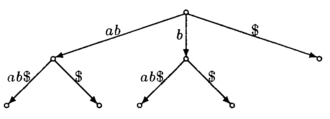
\includegraphics[width=2.5in]{st.png}
\caption{Suffix tree for string x=abab, \cite{Kurtz1999}.}
\label{suftree}
\end{figure}

Implementation of suffix tree suggested in \cite{Kurtz1999} has two structures: a reference structure which consists of an address pointing to a leaf, or to a branching node. branchinfo structure has the following items:
\begin{itemize}
  \item headposition: the head position of the branching node
  \item depth: the depth of the branching node
  \item suffixlink: the suffix link is always to a branching node
  \item firstchild: the reference to the first child
  \item branchbrother: the reference to the right brother, if this doesn't exist then it's \texttt{NULL}
\end{itemize}

 For the suffix tree in Figure \ref{suftree} the tables are shown in Figure \ref{tables}. 
\begin{figure}[!t]
\centering
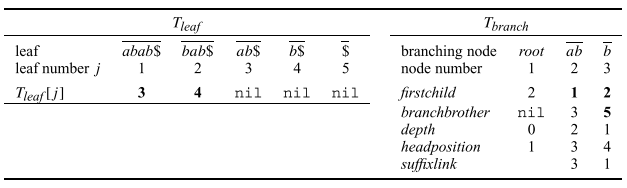
\includegraphics[width=3.5in]{tables.png}
\caption{Tables to store suffix tree for string x=abab, \cite{Kurtz1999}.}
\label{tables}
\end{figure}

The successors of a branching node are therefore found in a list whose elements are linked via the firstchild, branchbrother, and $T_{leaf}$ references. 

Every string occurring in a suffix tree $ST$ can uniquely be described in terms of the nodes and edges of $ST$. This is formalized in the notion of \textit{locations}:

\begin{mydef}
Let $ST$ be a suffix tree and $s \in words(ST)$. The \textit{location} of $s$ in $ST$, denoted by $loc_{ST}(s)$ is defined as follows:
\begin{itemize}
\item If $\overline{s}$ is an internal node, then $loc_{ST}(s)=\overline{s}$.
\item If $\overline{s}$ is a leaf in $ST$, then there is a leaf edge $\overline{u}\overset{v}{\rightarrow}\overline{s}$ in $ST$ and $loc_{ST}(s)=(\overline{u},v,\epsilon,\overline{s})$.
\item If there is no node $\overline{s}$ in $ST$, then there is an edge $\overline{u}\overset{vw}{\rightarrow}\overline{uvw}$ in $ST$ such that $s=uv, v\neq \epsilon, w\neq \epsilon$ and $loc_{ST}(s)=(\overline{u},v,w,\overline{uvw})$.
\end{itemize}
\end{mydef}

Following a path is the most important operation to search for MUMs. Function $TraverseSuffixTree$ describes this operation.
\begin{mydef}
Let $ST$ be a suffix tree. For each $s \in words(ST)$ and each string $w$ the function $scanprefix: locations(ST)\times\Sigma^{*}\rightarrow locations(ST)\times\Sigma^{*}$ is specified as follows: 
\begin{center}
$TraverseSuffixTree(loc_{ST}(s),w,ST)=(loc_{su},v)$,
\end{center}
where $uv=w$ and $u$ is the longest prefix of $w$ such that $su \in words(ST)$.
\end{mydef}

Moreover, it is very important to have an efficient access from $loc_{ST}(cy)$ to $loc_{ST}(y)$. This access is provided by a function suffixlink, that uses the suffix links of the inner nodes as a "shortcut".
\begin{mydef}
Let $ST$ be a suffix tree. Function suffixlink, $suffixlink:locations(ST)\ \left\lbrace root\right\rbrace\rightarrow locations(ST)$ is defined as:
\begin{center}
$suffixlink(\overline{s})=\overline{z}$
where $\overline{s}\rightarrow\overline{z}$ is the suffix link for $\overline{s}$
\[ suffixlink(\overline{u},av,w,\overline{uavw})= \left\{ 
  \begin{array}{l l}
    loc_{ST}(v) & \quad \text{if $\overline{u}=root$}\\
    rescan(\overline{z},av) & \quad \text{otherwise}
  \end{array} \right.\]
  where $\overline{u}\rightarrow \overline{z}$ is the suffix link for $\overline{u}$
\end{center}
\end{mydef}
Once we have defined the preliminaries in the MUM-problem, we need to answer the question: Where are the MUMs of $R$ and $Q$ of some minimum length $L$? We show the algorithm used to answer this question using a suffix tree, see Algorithm \ref{algST}.
\begin{algorithm}[]
  \label{algST}
  \SetKwInOut{Input}{input}
  \SetKwInOut{Output}{output}
  \SetKwData{R}{R}
  \SetKwData{Q}{Q}
  \SetKwData{ST}{ST}
  \SetKwData{Len}{L}
  \SetKwFunction{Length}{length}
  \SetKwData{Leaf}{leaf}
  \SetKwData{MUMs}{MUMs}
  \SetKwData{MUMcands}{MUMcands}
  \SetKwData{loc}{loc}
  \SetKwFunction{buildST}{buildST}
  \SetKwFunction{TraverseSuffixTree}{TraverseSuffixTree}
  \SetKwFunction{suflink}{suffixlink}
  \SetKwFunction{isRootNode}{isRootNode}
  \SetKwFunction{isLeafNode}{isLeafNode}
  \SetKwFunction{saveMUMcand}{saveMUMcand}
  \SetKwFunction{cleanMUMcand}{cleanMUMcand}
  \Input{\R, \Q, \Len}
  \Output{List of \MUMs of \Length$\geq$ \Len, with start position in \R and \Q and \Length}
  \Begin{
  \ST$\leftarrow$ \buildST{\R}\;
  \loc$\leftarrow$ \TraverseSuffixTree{$\Q[0]$,ROOT,\ST}\;
  \For{i=1 to $|Q|$}{
    \If{\isLeafNode{\loc} and \loc.length $\ge$ \Len }{
    \tcc{Leaf saves the position of a suffix in ST.}\;
        \If{$\R[\Leaf-1]\neq \Q[i-1]$}{
            \MUMcands$\leftarrow$ \saveMUMcand{$\R_{\Leaf}$,$i$,\Length}\;
        }
    }
  \eIf{\isRootNode{loc}}{
  \loc$\leftarrow$ \TraverseSuffixTree{$\Q[i+1]$,ROOT,\ST}\;
  }{
  \suflink{\ST,\loc}\;
  \loc$\leftarrow$ \TraverseSuffixTree{$\Q[i+1]$,\loc.node,\ST}\;
  }
  }
  \tcc{Get unique MUMs from list of MUM-candidates.}\;
  \MUMs$\leftarrow$ \cleanMUMcand{\MUMcands}
  }
  \caption{Search for MUMs in a suffix tree.}
\end{algorithm}

In Algorithm \ref{algST} there are two functions related to suffix tree. TraverseSuffixTree performs the traversal of the suffix tree with the current string  and it starts in some given node. suffixlink is a function which gets the suffix link from the current node pointed out by loc.node. If $b$ is an internal node $v$ of suffix tree, then the algorithm can follow its suffix link to a node $s(v)$. If $b$ is not an internal node, then the algorithm can back up to the node $v$ just above $b$. If $v$ is the root, then the search starts in root. But if $v$ is not the root, then the algorithm follows the suffix link from $v$ to $s(v)$.

\section{Suffix tree bottleneck}
\label{bottleneck}
Suffix tree is the archetypical index structure used in bioinformatics. For large-scale bioinformatics applications, however, memory consumption really becomes a bottleneck and a factor of higher latency. Moreover, the algorithm to search for MUMs involves comparing the search of a character to the character stored at a specific node at every level of the tree, and traversing a child node based on the comparison results. Only one node at each level is actually accessed, resulting in ineffective cache line utilization, to the linear storage of the tree. Result of the comparison is required before loading the appropriate next child node. Moreover, meanwhile the Algorithm \ref{algST} shows a $O(m)$ complexity by using suffix links, this feature has the disadvantage of a quite random access to the next node used to traverse the suffix tree. As a consequence a search for MUM typically involves a long-latency at each level of the tree, leading to ineffective utilization of the processor resources.

The best scenario (short-latency and no TLB/cache miss) in a search for MUM is a layout of a whole branch in a cache line size. The worst scenario (long-latency and TLB/cache miss) is a layout of only one branch read in a cache line size. In Figure \ref{suftree} the suffix tree is implemented with two tables as in Figure \ref{tables}. The layout of branch table has a poor temporal and spatial locality. 

Use of tables leaf and branch in Figure \ref{tables} helps to traverse a suffix tree, but since each branch node is implemented as a linked list this is a serious performance issue. In Figure \ref{stlocality} is shown some of the first nodes of a suffix tree, the squared numbers represent the number of node in the branch table. It can be shown that only a few nodes are contiguous, a contiguous linked list has a better locality and less latency.
 
\begin{figure}[hbtp]
\centering
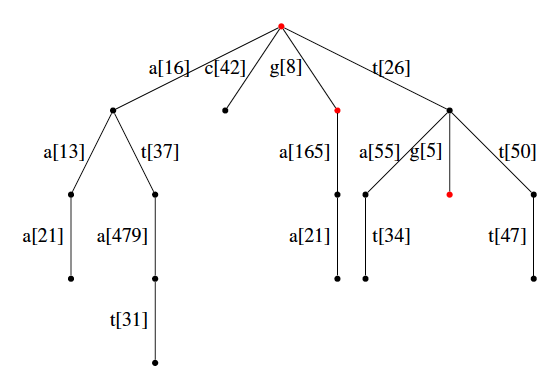
\includegraphics[scale=0.4]{st-locality.png}
\caption{First nodes of suffix tree. Red dots are adjacent memory references starting at root node.}
\label{stlocality}
\end{figure}

 The linked list have items in disjoint areas of memory. To traverse the list the cache lines cannot be utilized effectively. One could say that the linked list is cache line hostile, or that the linked list maximizes cache line misses. The disjoint memory will make traversing of the linked list slow because RAM fetching will be used extensively.

\subsection{Memory reference locality}
\label{locality}
This layout in Figure: \ref{tables} and \ref{stlocality} of a suffix tree and the random search of strings do not help to a better use of processor resources. The use of suffix links reduces the time complexity of a search for a MUM in a suffix tree but it is not very cache-friendly.

As a proof of a poor memory reference locality of this data structure, two experiments were carried out. The features of the computer used are: 2 Processor Intel(R) Xeon(R) E5645 @ 2.4GHz of 6 cores each one, 32KB L1 cache, 256KB L2 and 12MB L3 shared cache per socket. RAM: 96 GB. GCC 4.7.0 with OpenMP support + Linux.

The genomes used were a reference genome of 312Kbp\footnote{Measure unit in DNA genomes.} and 169Mbp, a query genome of 2.91Gbp and a minimum length of MUM of 20bp.

By using the memory heriarchy, we may overlap the latency of a random traversal in a suffix tree. The first experiment is with a small suffix tree (reference of 312Kbp), which is kept in the L3 cache (6MB of memory consumption for suffix tree), the query genome of 2.91Gbp is kept in main memory. The total time to search for MUMs was 149.58 seconds. The second experiment is with a bigger sufffix tree (reference of 169Mbp), which is kept in main memory (3380GB of memory consumption for suffix tree), the query genome of 2.91Gbp is kept in main memory. The total time to search for MUMs was 268.58 seconds. Furthermore, the functions in Algorithm \ref{algST} were profiled to get how many times are accessed in order to have an idea of the bottlenecks while traversing a suffix tree with suffix links. In experiment 1, 6.18\% of times the traversal started in the root of suffix tree. 60.38\% of times suffix links were used. By using suffix links 59.99\% of times the function rescan was used. These measures show how heavy and intensive is the used of suffix links and how it may degrade the performance. In experiment 2, 4.12\% of times the traversal started in the root of suffix tree. 66.47\% of times suffix links were used. In suffix links 69.23\% of times the function rescan was used.
 
\section{Enhanced traversal of Suffix Tree with SIMD instruction}
\label{enhanced}
In Section \ref{locality} is shown where the bottlenecks are in the MUMmer application. Function rescan involves to find the correct child to traverse with next node. However, because nodes are not arranged in a sequential way every access to a child node incurs in a high latency. To avoid this latency, a new arrangement is made in the suffix tree. So that suffix tree is traversed with algorithm breadth-first search and rearranged all nodes by depth level. This new order still has a latency but it is reduced the access time to child nodes because every child node is next to the other. If traversal of suffix tree requires to find the correct edge to continue, then this new order allows reading every child node, and its information, in a sequential way. Since we are focused in the search for MUMs time, this new layout of the suffix tree gives the opportunity to use SIMD instruction to find the correct child node as it is used in \cite{Kim2010}. 

To find the correct child in MUMmer application involves to read every child node and compare the first character against the current character in the query string. Therefore there are as many comparisons as children nodes are in the current parent node, because MUMmer application works with DNA the maximum number of children are 4 (a,c,g,t). 

With the current advances in SIMD instructions we can use a SIMD instruction to find the correct child with only one instruction. Then use the mask provided by SIMD instruction to get the offset from the first child and continue with the traversal of suffix tree. It is used a library\footnote{www.agner.org/optimize} which provides the functions to store, read and compare the first character of every child node.

An example of the use of this library to find the correct child:
\begin{verbatim}
Vec4i a(65,67,71,84);
Vec4i b(71,71,71,71);
Vec4i c = a==b; //c = (0,0,-1,0)
\end{verbatim}
 
The result of this comparison is used to compute the offset to find the correct child and continue with the lcp comparison of the current string in that edge and the query string.

\subsection{Experimental evaluation}
\label{experimental}
Goal is to reduce the execution time in the search for MUMs between a Reference and Query genome of some minimum length. To improve time, an evaluation of the search for MUMs algorithm was measured and findings are that the most time-consuming function of the algorithm is the traversal of suffix tree. A new layout of suffix tree is proposed and based on that layout the use of SIMD instructions to optimize the part of algorithm to find the correct child.

This little tweak allows having a reduction in the execution time. This reduction in time is because a whole while-loop is changed by a single SIMD instruction. Moreover, the contiguous children nodes have the advantage of reducing the latency and information stored in every child node can be loaded quicker.

To verify that our approach, can have a better performance to search for MUMs between a Query and Reference genome, we check that output of MUMmer and our approach has the same MUMs and with a reduction of execution time. This test was carried out in the following node:
\begin{itemize}
\item Hardware:  
\begin{itemize}
\item 2 Processor Intel(R) Xeon(R) E5645 @ 2.4GHz of 6 cores each one, 32KB L1 cache, 256KB L2 and 12MB L3 shared cache per socket.
\item RAM: 96 GB
\end{itemize} 
\item  Software: 
\begin{itemize}
\item Linux Kernel 2.6.32-220.el6.x86\_64 \#1 SMP
\item gcc 4.7.0 with OpenMP support
\end{itemize}  
\item Genomes:
  \begin{itemize}
    \item Reference: 
    \begin{itemize}
    \item Fly fruit genome, 169 [Mbp]
    \item Silkworm genome, 487.6 [Mbp]
\end{itemize} 
    \item Query: 
    \begin{itemize}
    \item Fly fruit genome, 166 [Mbp] 
    \item Red imported fire ant genome, 335.7 [Mbp]
    \end{itemize}
  \end{itemize}
\end{itemize}

In the first experiment, Figure \ref{s1}, it is shown a reduction in execution time of 17\% compared to the current implementation of MUMmer application. As it was explained before, this reduction in time is because children nodes are contiguous (less latency) and to find the correct child uses SIMD instructions (less instructions).
\begin{figure}[hbtp]
\centering
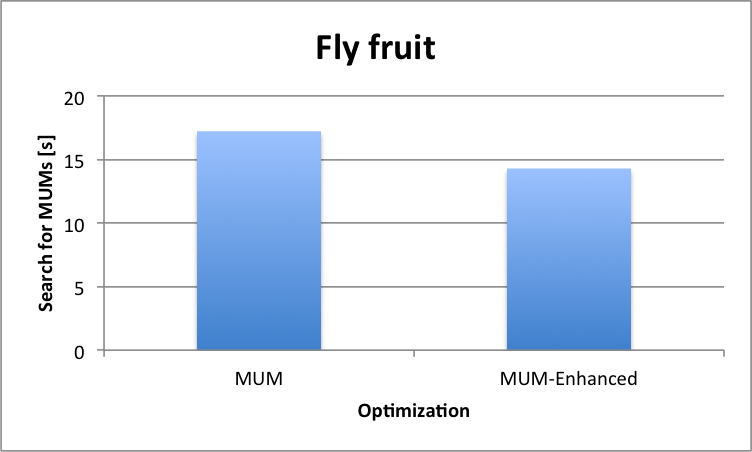
\includegraphics[scale=0.5]{serial1.png}
\caption{Comparison of execution time for Fly fruit 166 [Mbp]}
\label{s1}
\end{figure}

In the second experiment, Figure \ref{s2}, it has a bigger genome size and it is shown that we have a reduction in time of 17.06\%.
\begin{figure}[hbtp]
\caption{Comparison of execution time for Ant 335.7 [Mbp]}
\centering
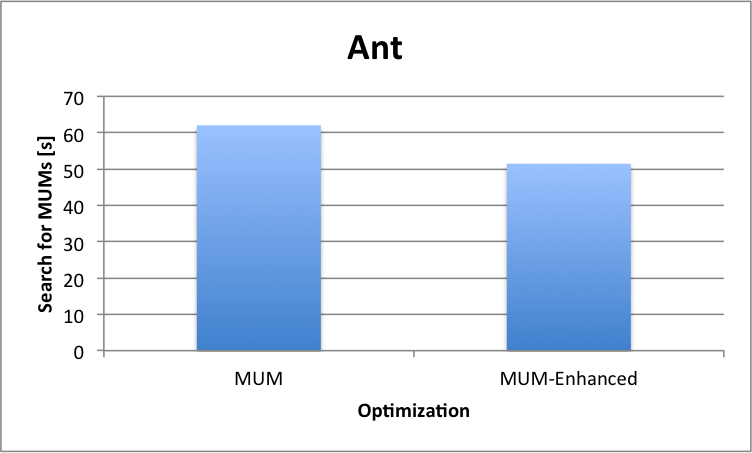
\includegraphics[scale=0.5]{serial2.png}
\label{s2}
\end{figure}

\section{Search for MUMs in Multicore architectures}
\label{multicore}
The sequential version of the MUM search between a Reference and Query genome trades high computation time when executed in a single machine. Previously the algorithm to search for MUMs was described. Now a proposal of a parallelization of MUM search within multi-core architecture is explained.

There are two resources to improve in this algorithm: Memory usage and CPU. The former was generally improved because it allows being executed in architectures where there is no memory restriction. To improve the performance of the algorithm a data-level parallelism technique is deployed.

This technique is divided in three phases following:
\begin{enumerate}
\item Splitting query genome data (chunks) according to the number of available cores using 1 thread per core. Chunk size is computed with the total of threads used, thus the chunk size is fixed.
\item Parallel execution of the task of Algorithm \ref{algST} for every chunk, after finishing its task every thread has its own list of MUM-candidates.
\item Get the final list of MUMs from every MUM-candidate list of all threads.
\end{enumerate}
To get a MUM requires an important feature its uniqueness. Uniqueness can only be found when a whole genome is checked, see Figure \ref{Whole-MUM}. If some part of it is only evaluated we could miss the rest of the genome. In other words, after finding MUMs within a chunk it is not possible to determine if the MUM found is or not a "unique" MUM, globally in the query genome,  because these MUMs are unique only in the chunk that has been read, the rest of the genome it is not known until all query genome has been read. In Figure \ref{Whole-MUM} is shown the consequences of using chunks for query genome. Meanwhile we may speed up the MUM search we need to deal with the discard of MUM-candidates which are not a real MUM. So that, after finding all MUM-candidates for every thread we need to verify which of MUM-candidates are MUMs.

\begin{figure}[htb]  
\begin{center} 
  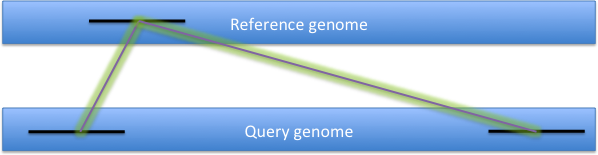
\includegraphics[width=6cm,height=3cm]{Whole-MUM.png}
\end{center} 
\caption{MUM in reference genome but not in query genome.} 
\label{Whole-MUM} 
\end{figure}

Phase 3 extracts the list of MUM from the set of MUM-candidates of every chunk in the query genome. In order to get the real MUMs we filter MUM-candidates that are overlapped by bigger MUM-candidates.
\subsection*{Implementation} 
\label{implementation}
\subsubsection*{Split query genome}  
As it was previously explained, the approach is to use a fixed size division of query genome. To split query genome the algorithm needs to know in advance how many chunks will be used (one thread/one chunk). Then every chunk is computed with two pointers (left and right end) which points out query genome in main memory.
\subsubsection*{Finding MUMs}
The parallelization is carried out with OpenMP, the Algorithm \ref{algST} is applied for every chunk. The algorithm to search for MUMs is a process which can be executed without any data dependency. 

Firstly, from Algorithm \ref{algST} some variables are shared among the threads in our OpenMP implementation: Suffix Tree, Reference genome and Query genome. Secondly, some variables are private for every thread: the location pointer to Suffix Tree, the pointer to the chunk of Query genome assigned to each thread and the array of MUM-candidate type.

\subsection{Experimental evaluation in Multicore archictectures} 
As it was described in Section \ref{experimental}, same node is used to measure the execution time by using the previous naive technique.

In Figure \ref{mthrd} is shown two experiments were the naive technique is deployed with OpenMP and one with the enhanced traversal of suffix tree. In first experiment, Fly fruit, a reduction in execution time is about 30\% compared to naive technique. This reduction in time is because the new layout in suffix tree provides a better locality and the reduction of instructions with the SIMD instructions. In second experiment, Ant, there is a minor reduction with naive technique about 27\%. However, this second experiment shows a better use of resources in multithreading processors with bigger genomes. The speedup is 34\% better in the SIMD technique with 24 threads.
\begin{figure}[hbtp]
\centering
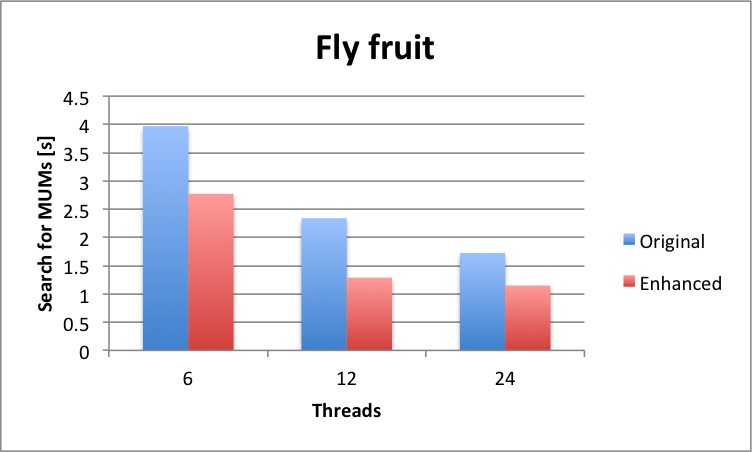
\includegraphics[scale=0.5]{multithread1.png}
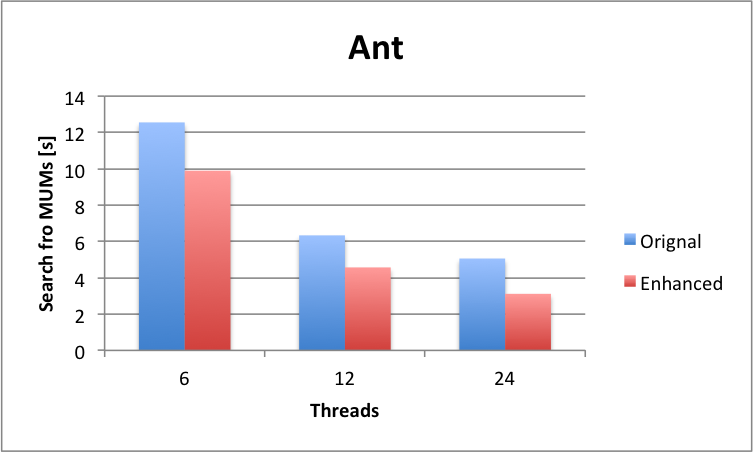
\includegraphics[scale=0.5]{multithread2.png}
\caption{Comparison of optimization in Multicore architectures.}
\label{mthrd}
\end{figure}
Goal is to reduce the execution time to search for MUMs. Therefore, experiments and measures with multicore architectures are focused in the search for MUMs algorithm, and more in detail in the traversal of suffix tree (main bottleneck in Algorithm \ref{algST}).
\section{Conclusion}
\label{conc}
Traverse of suffix tree and use of suffix links are bottlenecks for a better processor performance. In suffix trees larger than the Last Level of Cache, the performance is dictated by the number of cache lines loaded from the memory, and the hardware features available to hide latency due to potential TLB and Last Level of Cache misses. Firstly, an enhanced traversal of suffix tree for a single thread shows a better use of processor resources and a reduction in search time. Secondly, a multicore technique is explained and it is compared with the enhanced traversal of suffix tree which has a better speedup.

Traversal of suffix tree is the main bottleneck in the MUM-problem and it has been given an optimization with SIMD instructions in order to reduce the execution time. However, there are some improvements to be done. For instance, the lcp comparison at each node can be done with SIMD instructions and to have a reduction in execution time.

Moreover, random traversal of suffix tree could be avoided by using some kind of scheduler to traverse suffix tree in a top-down fashion and taking advantage of data locality in last level of cache.
\section*{Acknowledgment}
This work was supported by grant from "Ejecuci\'on eficiente de aplicaciones multidisciplinares: nuevos desaf\'ios en la era multi/many core", with reference TIN2011-28689-C02-01.

% trigger a \newpage just before the given reference
% number - used to balance the columns on the last page
% adjust value as needed - may need to be readjusted if
% the document is modified later
%\IEEEtriggeratref{8}
% The "triggered" command can be changed if desired:
%\IEEEtriggercmd{\enlargethispage{-5in}}

\bibliographystyle{IEEEtran}
\bibliography{references}
\end{document}


